%Objectives
\section{Objectives}
\label{af:o}

\subsection{Arc Flash Study Objectives}
\label{af:o:afso}

The study results shall be basis for implementation of an Arc Flash Hazard Program, that will meet regulation CSA Z462 as well as IEEE-1584.
\\
\\
Arc flash hazards can result from many factors, including dropped tools, accidental contact with electrical systems, build up of conductive dust, corrosion and improper work procedures. An arc is produced by flow of electrical current through ionized air after an initial flash over or short circuit, resulting in a flash that can cause significant heating and burn injuries to occur. 
\\
\\
Arc faults can cause serious injury or death to workers. At the initiation of an arc fault, tremendous energy can be released in a very brief time. Metal conductor parts can vaporize resulting in hot vapors and hot metal being violently spewed. The thermal energy can result in severe burns to workers caused by direct
exposure or clothing ignition.
\\
\\
Historically, the Electrical Safety Code and other safety codes have been primarily concerned with protection from fire, electrocution, and shock hazard.  Arc flash hazards were not addressed. This is changing.
\\
\\
Canadian Standards Association (CSA) Z462 standard and Institute of Electrical and Electronics Engineers (IEEE) 1584 2002, provide guidance on implementing appropriate safety procedures to limit Arc Flash Hazard.
\\
\\
OSHA considers CSA Z462 a consensus industry standard for assessing arc flash standards. Under this legislation, the employer is responsible to assess the hazards in the work place; Select, have, and use the correct PPE and Document the assessment.
\\
\\
OSHA considers Arc Flash assessments that follow CSA Z462, in compliance with OSHA requirements, and the accepted practice to protect workers from electrical safety hazards.
\\
\\
To implement a successful Arc Flash Hazard prevention program, an Arc Flash study shall be performed to in a manner that satisfies the regulation CSA Z462 as well as IEEE-1584.
\\
\\
For each selected location of your power distribution system, the Arc Flash analysis shall determine the Incident Energy, Arcing Fault Clearing Time; Limits of approach, 
Working Distance, Incident Energy, Clothing Class required and Hazard area classification.
\\
\\
The objective of the Analysis is to determine a number of factors that directly affect the Arc Flash Hazard:
\\
\\
\textbf{Incident Energy Exposure }\\   
This is the amount of thermal incident energy to which the worker's face and chest could be exposed at working distance during an electrical arc event. Incident energy is measured in joules per centimeter squared (J/cm2) or calories per centimeter squared (cal/cm2). 
\\
\\  
\textbf{Flash Protection Boundary }\\   
The flash protection boundary is an approach limit at a distance from exposed live parts or enclosed live parts if operation, manipulation, or testing of equipment creates a potential flash hazard, within which a person could receive a second degree burn if an electrical arc flash were to occur. A worker entering the flash protection boundary must be qualified and must be wearing appropriate PPE. The Flash Protection Boundary is required to be calculated by CSA Z462. 
\\
\\ 
\textbf{Level of PPE} \\   
This is the minimum level of Personal Protective Equipment in calories per centimeter squared, as evaluated in IEEE Standard 1584, with the intent to protect the worker from the thermal effects of the arc flash at 18 inches from the source of the arc.
\\
\\		
\textbf{Working Distance}\\
Closest distance to a worker's body excluding arms and hands, which would be exposed to the arc.
\\
\\		
\textbf{Clothing Class}\\
Minimum clothing class designed to protect a worker from second degree burns.
\\
\\
The following Table outlines the current standards:
\\
\begin{center}

\textbf{Minimum Thermal Recommended Protection}\\
(Based on CSA Z462 Table 5 pg. 47-48)

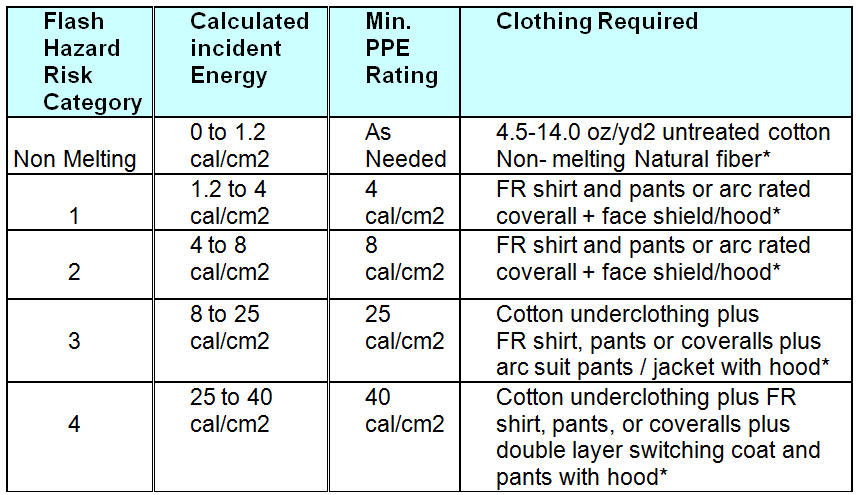
\includegraphics[width=5in, keepaspectratio=true]{../Images/Clothing.png} \\

\end{center}

\noindent *Note: In addition to clothing FR protective equipment is required as needed. Please see table 5 in CSA Z462 standard for further information. This can include items such as FR rated hard hats with inserts, safety glasses/goggles, hearing protection, leather safety shoes/gloves. Etc.

\pagebreak

\noindent The Arc Flash Analysis is merely a first step in implementing an Arc Flash Hazard Management Program.  The results of the study shall be further utilized in steps such as:\\

\begin{itemize}
\item	Implement the results of the Arc Flash Analysis - Modify your power distribution system parameters as needed (change settings on the protective relays/breakers, replace fuses etc.)
\\
\item	Implement a comprehensive labeling program - Identify all Electrical Equipment in the plant, including sources of power and limits of approach  
\\
\item	PPE and Training - Provide instructions and Personal Protective Equipment to all personnel that will be operating major electrical equipment.
\\
\item	Modify operating procedures (where practical) - change in switching arrangements, add remote tripping/closing to selected breakers, use long operating arms etc.
\end{itemize}